% !TeX spellcheck = en_GB
\documentclass[handout]{beamer}\mode<presentation>{\usetheme{AMSCesenaPurpleAndGold}}
%\documentclass[presentation]{beamer}\mode<presentation>{\usetheme{AMSCesenaBleu}}
%%%%

\usepackage{common}
\usepackage{courses}

\title{Environment Setup Tutorial}
%
\subtitle[SD]
{Distributed Systems / Technologies\\\scriptsize Sistemi Distribuiti / Tecnologie}
%
\author[Ciatto \and Omicini]
{\alert{Giovanni Ciatto} \and Andrea Omicini\\
\texttt{giovanni.ciatto@unibo.it \and andrea.omicini@unibo.it}}
%
\institute[DISI, Univ. Bologna]
{Dipartimento di Informatica -- Scienza e Ingegneria (DISI)\\\textsc{Alma Mater Studiorum} -- Universit{\`a} di Bologna a Cesena}
%
\date[A.Y. 2020/2021]{Academic Year 2020/2021}

\setbeamercovered{transparent}

\AtBeginSection[]
{
	\begin{frame}[c]\frametitle{Next in Line\ldots}
	%		\begin{multicols}{2}
			\tableofcontents[sectionstyle=show/shaded, subsectionstyle=show/hide, subsubsectionstyle=hide/hide]
	%		\end{multicols}
	\end{frame}
}

\begin{document}

\maketitle

\begin{frame}[c]\frametitle{Outline}
	\tableofcontents[sectionstyle=show/show, subsectionstyle=show/show, subsubsectionstyle=hide/hide]
\end{frame}

\section{General Recommendations}

\begin{frame}[allowframebreaks]
\frametitle{General Recommendations}

    \begin{itemize}
        \item in the general case we kindly suggest to \alert{use the Lab machines} when attending some Lab lesson \alert{in presence}, instead of your own laptops
        \item this is \alert{preferred} since we cannot guarantee your laptop to be properly configured 
        \item furthermore, laptops connected to ALMAWIFI cannot directly communicate with Lab machines because of firewall rules we cannot change, thus potentially limiting the impact of our exercises
        \item finally, we would like to avoid wasting time configuring it \emph{during} the lesson: that time is entirely needed to present the course contents
        \item of course, we will be glad of helping you configuring your laptops \alert{before} or \alert{after} any lecture, or by means of the \alert{students' forum} 
    \end{itemize}
    
    \framebreak
    
    \begin{itemize}
        \item in order for the Lab exercises to be reproducible on your laptops or home computers, you need to have a \alert{correctly configured environment}
        \item you may also be asked to perform some basic tasks such as discovering some machine IP address or, in general, using the console
        \item this tutorial will help you configuring your computer 
        \item this tutorial will teach you some basic operations from the command line
        \item[!] please consider reading these slides \alert{before} asking for help
        \begin{itemize}
            \item you are master students now and you can be autonomous :)
        \end{itemize}
    \end{itemize}
    
\end{frame}

\section{Ensuring Your Configuration is Correct}

\begin{frame}[c,allowframebreaks]
\frametitle{Your Configuration is Correct}

	\begin{enumerate}

    \item a correct configuration includes the following software runtimes:
    %
    \begin{itemize}
        \item \href{https://www.oracle.com/java/technologies/javase-jdk15-downloads.html}{Java Development Kit (JDK) $\geq 10$} 
		\begin{itemize}
			\item \alert{please avoid JDK versions $< 10$}
		\end{itemize}
        \item \href{https://gradle.org/releases}{Gradle $\geq 6.5.0$}
        \item \href{https://git-scm.com}{Git $\geq 2.25.0$}
    	\item \emph{(optional)} \href{https://www.docker.com/products/docker-desktop}{Docker Community Edition (CE) $\geq 19.0.0$}
    \end{itemize}

	\item ensure they are installed or install them if they are not
	%
	\begin{itemize}
		\item please notice that Gradle required Java to be installed
	\end{itemize}
    
    \framebreak
    
    \item if your configuration is correct, the following commands should provide an output similar to the one shown in this slide:
    %
    \begin{itemize}
        \item[\$] \texttt{java -version}
        \begin{itemize}
            \item[$\rightarrow$] \texttt{openjdk 15 2020-09-15}
            \item[] \texttt{OpenJDK Runtime Environment (build 15+36-1562)}
            \item[] \texttt{OpenJDK 64-Bit Server VM (build 15+36-1562, mixed mode, sharing)}
        \end{itemize}
        
        \item[\$] \texttt{javac -version}
        \begin{itemize}
            \item[$\rightarrow$] \texttt{javac 15}
        \end{itemize}
        
        \item[\$] \texttt{gradle --version}
        \begin{itemize}
            \item[$\rightarrow$] \texttt{Gradle 6.X.Y}
            \item[] \ldots
        \end{itemize}
        
        % \item[\$] \texttt{docker --version}
        % \begin{itemize}
        %     \item[$\rightarrow$] \texttt{Docker version 17.X.Y-ce, build ZZZ}
        % \end{itemize}
        
        \item[\$] \texttt{git --version}
        \begin{itemize}
            \item[$\rightarrow$] \texttt{git version 2.25.X.Y}
        \end{itemize}
    \end{itemize}
	%
	\framebreak
    %
    For instance, on Windows:
    %
    \begin{center}
        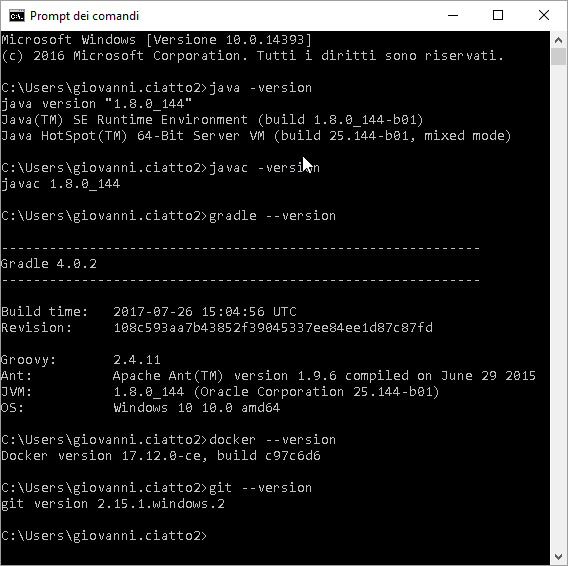
\includegraphics[width=.4\linewidth]{res/img/console_versions.png}
    \end{center}
    %
    \alert{If you get any trouble}, ensure the aforementioned software is correctly installed AND the following environment variables are properly set.
    
    \framebreak
    
    \item you must ensure the \texttt{JAVA\_HOME} and \texttt{GRADLE\_HOME} environment variables are properly set
    %
    \begin{itemize}
    	\item they should respectively point to the paths where \texttt{JDK} and Gradle are installed
    \end{itemize}
    
    \vspace{.5cm}
    
    \item for instance, you can check them by running the following console commands:
    %
    \begin{itemize}
        \item[$>$] \texttt{echo \alert{\%}JAVA\_HOME\alert{\%} \& echo \alert{\%}GRADLE\_HOME\alert{\%}}
        \begin{itemize}
            \item[$\rightarrow$] \texttt{C:$\backslash$Program Files$\backslash$Java$\backslash$jdk\_15.X\_Y} \hint{your paths may}
            \item[] \texttt{C:$\backslash$Program Files$\backslash$Gradle$\backslash$gradle-6.X.Y} \hint{be different}
        \end{itemize}
    \end{itemize}
    %
    on Windows-based systems, or
    %
    \begin{itemize}
        \item[\$] \texttt{echo \alert{\$}JAVA\_HOME ; echo \alert{\$}GRADLE\_HOME}
        \begin{itemize}
            \item[$\rightarrow$] \texttt{/usr/lib/jvm/java-15-openjdk-amd64/}\hint{your paths may}
            \item[] \texttt{/opt/gradle/gradle-6.X.Y}\hint{be different}
        \end{itemize}
    \end{itemize}
    %
    on Unix-based systems.
    
   \framebreak
    
   \item then, you must ensure your \texttt{PATH} environment variable contains the paths  where the aforementioned runtimes are installed into. 
	%
	\begin{itemize}
		\item[!] if you succeeded with the previous steps, this should be ok, but please double check :)
	\end{itemize}
	%    
    \vspace{.5cm}
    %
    For instance, you can check it by running the following console commands:
    %
    \begin{itemize}
        \item[$>$] \texttt{echo \alert{\%}PATH\alert{\%}}
        \begin{itemize}
            \item[$\rightarrow$] \texttt{<path1>}\alert{;}\texttt{<path2>}\alert{;}$\ldots$\alert{;}\textit{\texttt{<java\_home>$\backslash$bin}}\alert{;}$\ldots$\alert{;}\textit{\texttt{<gradle\_home>$\backslash$bin}}\alert{;}$\ldots$
        \end{itemize}
    \end{itemize}
    %
    on Windows-based systems, or
    %
    \begin{itemize}
        \item[\$] \texttt{echo \alert{\$}PATH}
        \begin{itemize}
            \item[$\rightarrow$] \texttt{<path1>}\alert{:}\texttt{<path2>}\alert{:}$\ldots$\alert{:}\textit{\texttt{<java\_home>/bin}}\alert{:}$\ldots$\alert{:}\textit{\texttt{<gradle\_home>/bin}}\alert{:}$\ldots$
        \end{itemize}
    \end{itemize}
    %
    on Unix-based systems.
    
    \framebreak
    
    \item ensure your local Git properties \alert{\texttt{user.name}} and \alert{\texttt{user.email}} are properly set by running the following commands:
    %
    \begin{itemize}	
    	\item[\$] \texttt{git config --global --get user.\alert{name}}
    	%
    	\begin{itemize}	
    		\item[$\rightarrow$] \texttt{\textit{<your name>}}    		
    	\end{itemize}
    	
    	\item[\$] \texttt{git config --global --get user.\alert{email}}
    	%
    	\begin{itemize}	
    		\item[$\rightarrow$] \texttt{\textit{<name>}.\textit{<surname>}[\textit{<number>}]@\alert{studio.unibo.it}}    		
    	\end{itemize}
    
    	\vspace{.5cm}
    	
    	\item In case they are not, you can set them by means of the following command
    	%
    	\begin{itemize}	
    		\item[\$] \texttt{git config --global \texttt{\textit{<property\_name>}} \alert{"}\texttt{\textit{<value>}}\alert{"}}		
    	\end{itemize}
    \end{itemize}
    
	\end{enumerate}

\end{frame}

\section{Create the Required Accounts}

\begin{frame}\label{configure-accounts}
\frametitle{Create the Required Accounts}
    
    For this course, you will need to:
    %
    \begin{enumerate}
        \item be enrolled into the course e-learning web-page
        \begin{itemize}
            \item \url{https://virtuale.unibo.it/course/view.php?id=18643}
            \item you should be already enrolled because of your courses plan
            \item if you are not, you can enroll providing the key \alert{\texttt{2021SD}}
        \end{itemize}
        
        \item register a GitLab account using your \alert{\texttt{x.yN@studio.unibo.it}} email address
        \begin{itemize}
            \item \url{https://gitlab.com/users/sign_in\#register-pane}
            \item please use \texttt{x.yN} as username, if possible
        \end{itemize}
        
		\item register a Docker Hub account using your \alert{\texttt{x.yN@studio.unibo.it}} email address
		\begin{itemize}
			\item \url{https://hub.docker.com/}
			\item please use \texttt{xyN} as Docker ID, if possible
		\end{itemize}
        
        \item request access on the Distributed Systems GitLab group for the A.Y. 2020/2021:
        %
        \begin{itemize}
            \item \url{https://gitlab.com/pika-lab/courses/ds/ay2021}
        \end{itemize}
        
    \end{enumerate}
    
\end{frame}

\section{Operations}

\subsection{Importing Your (Git) Project in Eclipse}

\begin{frame}[c,allowframebreaks]
\frametitle{Importing Your (Git) Project in Eclipse} 
    Suppose you want to import your Git \texttt{http://gitwhatever.com/path/to/\alert{my-project}} project in Eclipse:
    %
    \begin{enumerate}
        \item clone your project within the \texttt{\alert{my-dir}} directory:
        %
        \begin{itemize}
            \item[!] Ensure \texttt{my-dir} is NOT an Eclipse workspace
            \item[\$] \texttt{cd \alert{my-dir}}
            \item[\$] \texttt{git clone http://gitlab.com/path/to/X} 
        \end{itemize}
        
        \item \textbf{start Eclipse and choose \texttt{\alert{my-dir}} as the workspace directory}
        
        \item if the cloned repository contains a Gradle project, skip to slide \ref{import-gradle-project}
        
        \item import the existing project into the workspace, if possible:
        %
        \begin{enumerate}
            \item click on \texttt{File} a menu should appear
            \item click on \texttt{Import...} a dialog window should appear
            \item from that dialog, open the \texttt{General} folder
            \item select the \texttt{Existing Projects into Workspace} and click on \texttt{Next}
            \item ensure the \texttt{Select root directory} field is selected
            \item click on the \texttt{Browse...} button and select the \texttt{\alert{my-dir}} directory (i.e.,  the current workspace)
            \item if your cloned project \texttt{\alert{my-project}} is visible within the \texttt{Projects} area, select it and hit the \texttt{Finish} button
            \item otherwise, Git is not tracking Eclipse's project files and you must import the project the hard way (next step)
        \end{enumerate}
        
        \item if the previous procedure fails, close the \texttt{Import} dialog and
        %
        \begin{enumerate}
            \item click on \texttt{File} a menu should appear
            \item select the \texttt{New > Java Project} entry
            \item type \texttt{\alert{my-project}} within the \texttt{Project name} field
            \item hit the \texttt{Finish} button
        \end{enumerate}
        
        \item if no procedure succeeded you can call for help :)
        
    \end{enumerate}
\end{frame}

\subsection{Importing Your (Gradle) Project in Eclipse}

\begin{frame}[allowframebreaks]
\frametitle{Importing Your (Gradle) Project in Eclipse}
\label{import-gradle-project}

    Suppose you want to import your local Gradle project (whose main directory is \texttt{/path/to/\alert{my-dir}/gradle-project}/) in Eclipse:
    
    \begin{enumerate}
        \item ensure the value of the  \texttt{rootProject.name} property in \texttt{gradle-project/\alert{settings.gradle}} is equals to the name of the project's main directory (i.e., \texttt{gradle-project} in this example)
        
        \item \textbf{start Eclipse and choose \texttt{\alert{my-dir}} as the workspace directory}
        
        \item import the existing project into the workspace, if possible:
        %
        \begin{enumerate}
            \item click on \texttt{File} a menu should appear
            \item click on \texttt{Import...} a dialog window should appear
            \item from that dialog, open the \texttt{Gradle} folder
            \item select the \texttt{Existing Gradle Project} and click on \texttt{Next}
            \item specify \texttt{gradle-project} as project name and \texttt{/path/to/my-dir/gradle-project} as project location, then click on \texttt{Next}
            \item activate the \texttt{Override workspace settings} check-box and ensure the \texttt{Gradle wrapper} combo-box is selected, then click on \texttt{Next}
            \item click on \texttt{Finish}
            %
            \begin{itemize}
                \item if nothing happens call for help
            \end{itemize}
        \end{enumerate}
        
    \end{enumerate}
    
\end{frame}

\subsection{Submitting Your Exercise}

\begin{frame}%[allowframebreaks]
\frametitle{Submitting Your Exercise}

    \begin{itemize}

        \item sometimes, you may be asked to submit some exercises
        
        \item in such cases, you will usually clone them from a GitLab repository
        %
        \begin{itemize}
            \item so please \textbf{request access} here: \url{https://gitlab.com/das-lab/courses/ds/ay2021} in order to get the right to push your commits
        \end{itemize}
        
        \item if you are asked to submit your solution to a given exercise, you can only do so by \alert{pushing} your code on a particular branch of the GitLab repository of that exercise
        
        \item the branch must be named as follows:
        \begin{itemize}
            
            \item \texttt{submissions/\alert{\textit{name.surnameN}}}%, in case you are submitting on time
            % \item \texttt{late-submissions/\alert{\textit{name.surnameN}}}, otherwise
            
            \vspace{.3cm}
        
            % \item[!] The definition of ``on time'' may vary but it usually means ``before the next Lab lecture''
            
            % \item[!] Of course, your push right on the \texttt{submissions/*} branches will eventually be deactivated
            
            \vspace{.3cm}
            
            \item[$\downarrow$] Example on the next slide

        \end{itemize}

    \end{itemize}
\end{frame}

\begin{frame}[allowframebreaks]
\frametitle{Exercise Workflow Example}

    \begin{enumerate}
        \item clone the exercise repository
        %
        \begin{itemize}
            \item[\$] \texttt{git clone https://gitlab.com/das-lab/courses/ds/aa1920/\alert{\textit{exericse\_name}}}
        \end{itemize}
        
        \item jump into the project directory
        %
        \begin{itemize}
            \item[\$] \texttt{cd \alert{\textit{exericse\_name}}}
        \end{itemize}
        
        \item create a novel submission branch:
        %
        \begin{itemize}
            \item[\$] \texttt{git checkout -b submissions/\textit{\alert{name.surnameN}}}
        \end{itemize}
        
        \item repeat until exercise completion:
        %
        \begin{enumerate}
            \item do some work
            \item add the edited files to the stage
            %
            \begin{itemize}
                \item[\$] \texttt{git add \textit{\alert{edited\_file1}}, \textit{\alert{edited\_file1}}, \ldots}
            \end{itemize}
            \item commit the staged files 
            %
            \begin{itemize}
                \item[\$] \texttt{git commit -m "\textit{\alert{a message here}}"}
            \end{itemize}
            \item push on the \texttt{submissions/\textit{\alert{name.surnameN}}} branch
            %
            \begin{itemize}
                \item[\$] \texttt{git \alert{push}}
            \end{itemize}
        \end{enumerate}
        
    \end{enumerate}

\end{frame}

\subsection{Discovering Your Machine IP Address}

\begin{frame}[allowframebreaks]
\frametitle{Discovering Your Machine IP Address(es)} 


	In several scenarios you may be required to discover your machine current IP address
	%
	\columnsHHt{
		\begin{itemize}
		    \item on Windows, you can do it by prompting:
		    %
		    \begin{itemize}
		        \item[$>$] \texttt{ipconfig}
		    \end{itemize}
		\end{itemize}
		%
		\begin{center}
			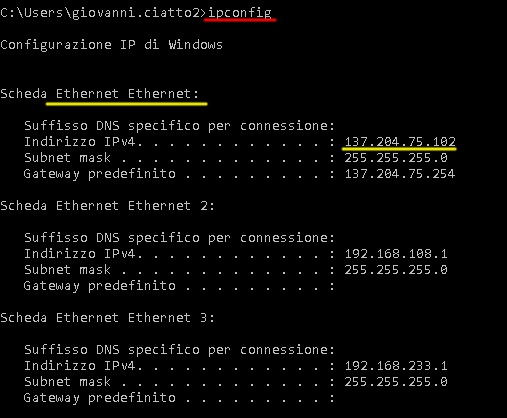
\includegraphics[width=.9\linewidth]{res/img/ipconfig.png}
		\end{center}
	}{%\framebreak
    \begin{itemize}
	    \item whereas, on Unix, you can do it by prompting:
	    %
	    \begin{itemize}
	        \item[\$] \texttt{ifconfig}
	    \end{itemize}
	\end{itemize}
	%
	\begin{center}
		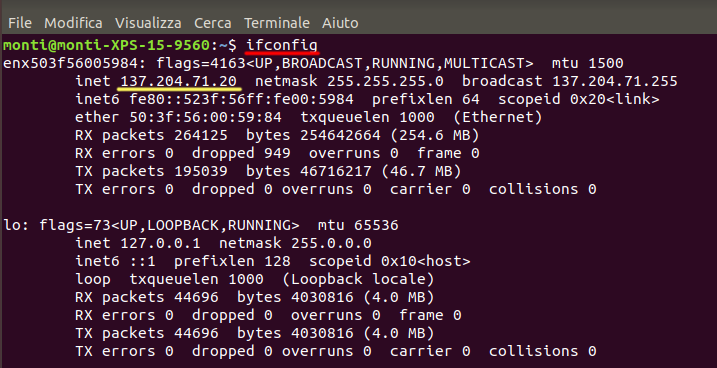
\includegraphics[width=.9\linewidth]{res/img/ifconfig.png}
	\end{center}
	}
    
    \framebreak
    \begin{itemize}
    \item keep in mind that:
    %
    \begin{itemize}
    	\item IP addresses are often dynamically assigned by means of DHCP, so \alert{do not expect} you machine to always be assigned with the same IP address
    	\item IP addresses are usually NATted, thus they are not accessible from the Internet
    	\item UniBo's IP addresses are \emph{usually} in the \texttt{137.204.xx.xx} form
    	\item Docker \emph{usually} assign IPs to containers in from the \texttt{172.xx.xx.xx} range
    \end{itemize}
	\end{itemize}

\end{frame}

\subsection{Configure Your Own Computer}

\begin{frame}
\frametitle{Configure Your Own Computer}

	Some useful tutorials:
	%
	\begin{itemize} 
		
		\item \href{https://docs.gradle.org/current/userguide/installation.html\#installing_manually}{How to install Gradle on Windows, Mac OS, or Linux}
		
		\item	 \href{https://confluence.atlassian.com/doc/setting-the-java_home-variable-in-windows-8895.html}{Hot to set the \texttt{JAVA\_HOME} environment variable on Windows}
		%
		\begin{itemize}
			\item other environment variables can be set in a similar way
		\end{itemize}
		
		\item \href{https://www.java.com/en/download/help/path.xml}{How to edit the \texttt{PATH} environment variable on Windows or Mac OS}
		%
		\begin{itemize}
			\item instructions for Mac OS are ok for Linux too
		\end{itemize}
	
 		\item \href{https://docs.microsoft.com/it-it/virtualization/hyper-v-on-windows/quick-start/enable-hyper-v}{How to enable Hyper-V on Windows}
	
		\item \href{https://git-scm.com/book/en/v2/Customizing-Git-Git-Configuration}{How to set up Git properties}
	\end{itemize}

	\begin{block}{}
		In case of troubles, you can post on the \href{https://virtuale.unibo.it/mod/forum/view.php?id=331530}{Students' Forum} \alert{describing your issues}, your computer's features, and the steps you already performed :)
	\end{block}

\end{frame}

\subsection{Troubleshooting}

\begin{frame}\label{troubleshooting}
\frametitle{Troubleshooting} 
	\begin{itemize}
		\item in case your PC runs Windows 10 Home or some former version of Windows, you can freely and legally get a Windows 10 Pro license \& self-installing image since you are an UniBo student
		%
		\begin{itemize}
			\item you must apply to \href{https://dreamspark.campusfc.unibo.it/}{UniBo's Microsoft Programme}
			\item it may require a few days for your account to be activated 
		\end{itemize}
	
		\vspace{.3cm}
	
		\item for other sorts of troubles, please create a post on the \href{https://virtuale.unibo.it/mod/forum/view.php?id=331530}{Students' Forum}
		
	\end{itemize}
\end{frame}

\maketitle

%%%%%%%%%%%%%%%%%%%%%%%%%%%%%%%%%%%%%%%%%%%%%%%%%%%%%%%%%%%%%%%%%%%%%%%%%%%%%%%
\end{document}
%%%%%%%%%%%%%%%%%%%%%%%%%%%%%%%%%%%%%%%%%%%%%%%%%%%%%%%%%%%%%%%%%%%%%%%%%%%%%%%%